Virtualization is a way for a data center to reduce cost and power by overcommitting and sharing system resources across disparate operating systems with common hardware.  
In a single server environment or HPC cluster there can be \emph{interference} \cite{paul} or \emph{system noise}\cite{tsafrir} caused by complex software layers (Application, OS, and Hardware), which contribute to poor application performance.  
The hypervisor, as well as multiple external guest virtual machines (Figure \ref{virtStack}), compete for system resources and add to this interference.  
The thesis is current performance tools in the virtual guests are unable to distinguish between performance problems in the guest machine and external interference.  Aggregating resource counters and statistics across all layers of virtualization can dynamically measure the interference from virtualization.

\indent Due to the cost savings and decreased physical administration overhead, Data Centers and Businesses are moving toward virtualized environments.  In 2008 Gartner’s showed that 12\% of hardware at data centers were virtualized, and then predicted that by 2013 61\% would be virtualized \cite{gartners}.   Additionally, research from Ramya and Edwin show tremendous growth in Platform As A Service (PAAS) where an entire system platform is dynamically provisioned in a cloud computing service \cite{ramya}.   Massive data centers are able to provide virtual systems, and manage large clusters of shared resources, for a fraction of the price of building a physical server for each customer.

On a physical server, we can assume the hardware speed is relatively static.  For a CPU we can measure in Mhz and Flops, and for a disk we can use IOPS and latency.  From this data, or even from a baseline application measurement, we can view the performance of our application through performance tools such as \emph{top}, \emph{iostat}, and \emph{sar} on a Linux OS, and \emph{Perfmon} or {Winperf} on a Windows OS.  When that system is virtualized, the availability of the virtual resources are dynamic.  At any time, the resource may (or may not) be available to the guest and the performance tools become nearly meaningless.  There is almost no way to distinguish between a poor running application, OS Kernel issue, or external interference.  From the Hypervisor view, there is no information about the guest applications, so there is no way to relate problems to a specific application.  Furthermore, the entity managing the hypervisor layer is likely a completely different organization than the entity managing the virtual guest. 

Since each guest machine only uses a portion of the available resources at any given time, the total resources allocated to all guest VMs can exceed the total physical resources \cite{huber2, amit, buell1}.   This idea of overcommitting resources is the same as preemptive multitasking, where multiple processes share a single CPU; and OS virtual memory, where the total memory available to applications exceeds the physical memory capacity.  In order to maximize resources, IT Data Centers overcommit the resources, with the hope that multiple virtual guest machines do not need all resources concurrently.  
Sharing resources uniformly can cause interference in virtualization.  This is due to the fact that most of the operations in a virtual guest are run against a virtual resource by the guest system and then also implemented against the physical hardware resource.  

Existing performance tools fall into three categories, but they are not adequate for current performance problems with virtualization.
First, profiling tools are available on limited platforms, and require significant guest kernel and hypervisor support, configuration, and coordination.  Additionally, profiling is a great tool for test and development, but may not be a great solution for production systems.  
Second, performance monitoring tools are readily available on most every operating system.  They are very valuable for physical hardware but they assume that the resources are constant.  The performance data provided when the resources are used by external systems is indistinguishable from a change in the application workload.
Finally, hypervisor tools can show each guest and the physical resources, but they do not have access to the applications in the guest.  There is no way to relate a problem seen in the hypervisor to specific processes in the guest or the guest kernel. 

\begin{figure}[!h]
  \begin{center}
  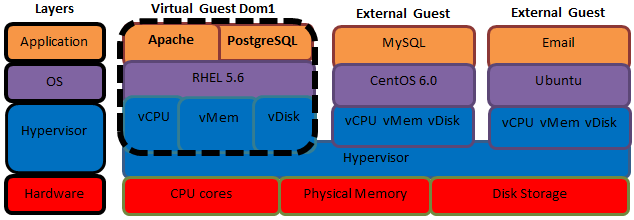
\includegraphics[width=6in]{images/LayersAll.png}
  \caption{In this example Domain 1 is running with some external systems.  The Xen hypervisor  divides, shares, and overcommits the physical resources between the 3 guest domains.  Each guest has access to virtual resources and not physical hardware.}
  \label{virtStack}
  \end{center}
\end{figure}

\indent This research presents a method for analyzing performance data at runtime in the guests and Virtual Machine Monitor (VMM).   With this framework we can detect the I/O interference by sharing physical and virtual I/O performance statistics between multiple guests.  We believe that this method can be extended to find interference from other resources.  This could significantly reduce time spent troubleshooting and analyzing performance problems in virtualized environments.

\indent This project will add the following contributions for virtualization:
\begin{enumerate}
\item \textbf{Layers} Define the layers of abstraction in virtual environments.
\item \textbf{Resources} Define the physical and virtual resources which need to be measured.
\item \textbf{Counters} Examine some common counters, and metrics which can measure resource utilization.
\item \textbf{Overhead} Design a method to measure the overhead of virtualization.
\item \textbf{Interference} Design a method to collect resource metrics at several layers and quantify the I/O interference from virtualization.
\item \textbf{Test Suite} Virtualization test suite that causes I/O interference and validates our design for detecting interference with I/O.
\end{enumerate}

\indent The rest of this document is organized as follows:  In section 2, we review a real problem example in a large data center, and the challenges faced with existing tools.  In section 3, we examine related works that have identified interference, root cause analysis, and the current state of tools used to analyze performance issues with virtualization.   In section 4 we define the needed data, a method to collect and analyze this data, and our test suite infrastructure.  Section 5 results shows the accuracy of our method on two different architectures.  We also explore other possible uses and what needs further investigation.
